
\documentclass[11pt,a4paper]{article}

\usepackage[margin=2.4cm]{geometry}
\usepackage{graphicx}
\graphicspath{{out/plots/}{../out/plots/}{out/data_analyze/}{../out/data_analyze/}{out/mermaid/}{../out/mermaid/}{figures/}}
\usepackage{amsmath, amssymb}
\usepackage{booktabs}
\usepackage{multirow}
\usepackage{float}
\usepackage{subcaption}
\usepackage{hyperref}
\usepackage{url}
\usepackage{caption}
\usepackage{listings}
\usepackage{xcolor}
\usepackage{siunitx}
\setlength{\emergencystretch}{3em}

\hypersetup{
  colorlinks=true,
  linkcolor=blue,
  urlcolor=blue,
  citecolor=blue
}
\hypersetup{pageanchor=false}

% ---------- Code listing style ----------
\lstdefinestyle{mystyle}{
  basicstyle=\ttfamily\small,
  breaklines=true,
  frame=single,
  columns=fullflexible,
  keywordstyle=\color{blue},
  commentstyle=\color{gray},
  stringstyle=\color{teal},
  showstringspaces=false
}
\lstset{style=mystyle}

\title{\textbf{Deep Learning for the Detection of \textit{Seizures}\\
in Electro-Encephalogram Signals}\\[4pt]
\large Project-Based Learning Report}
\date{\today}

\begin{document}
\begin{titlepage}
  \centering
  \vspace*{1cm}
  {\LARGE\textbf{Deep Learning for the Detection of \textit{Seizures in Electro-Encephalogram Signals}}\\[0.5cm]}
  {\large Project Report\par}
  \vspace{1.5cm}
  % Cover image: use main accuracy plot
  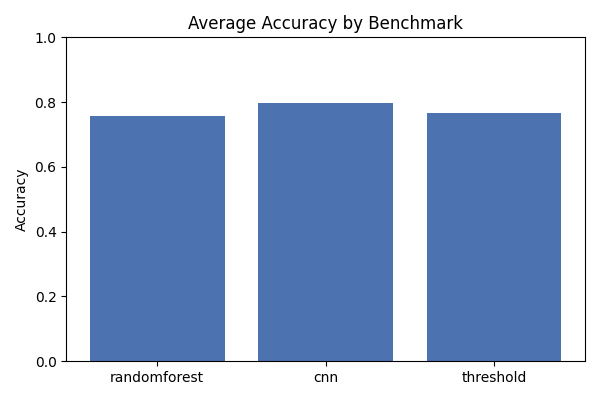
\includegraphics[width=0.7\linewidth]{average_accuracy.png}\\[1cm]
  \vfill
  \begin{tabular}{rl}
    Rubén Alba & NIU 1786494 \\
    Rohit Ranbawale & NIU 1744008 \\
    Michael Rienessl & NIU 1699828 \\
    Théotime Donnenfeld & NIU 1786565 \\
  \end{tabular}
  \vspace{1cm}\par
  Universitat Autònoma de Barcelona (UAB)\\
  \textbf{Course: Deep Learning}
  \vspace{0.5cm}\par
  \today
\end{titlepage}
\newpage

\begin{abstract}
\noindent
This report investigates the automated detection of epileptic seizures in EEG signals using four approaches:
a basic threshold-based algorithm operating on raw signal statistics, a random forest trained on handcrafted time-domain features, a one-dimensional convolutional neural network (CNN) trained on raw signal windows, and a recurrent LSTM that processes windows as temporal episodes.
EEG recordings from 24 patients are segmented into 1\,s windows, totalling \num{571905} samples (\num{3480} seizure windows) and evaluated under patient-level and seizure-level cross-validation.
The CNN achieves higher accuracy than the random forest, while the LSTM exploits the sequential structure of seizure episodes.
\end{abstract}

\tableofcontents
\hypersetup{pageanchor=true}
\newpage

\section*{Glossary}
\addcontentsline{toc}{section}{Glossary}
\label{sec:glossary}

\begin{description}
  \item[CNN] Convolutional neural network. Supervised patch-level classifier.
  \item[CV] Cross-validation. Here: 5-fold patient-level or seizure-level CV depending on model.
  \item[F1] F1 score. Harmonic mean of precision and recall: $2 \cdot \mathrm{precision} \cdot \mathrm{recall} / (\mathrm{precision} + \mathrm{recall})$.
  \item[FPR] False positive rate. Proportion of true negatives incorrectly predicted positive; $\mathrm{FP}/(\mathrm{TN}+\mathrm{FP})$.
  \item[LSTM] Long short-term memory. Recurrent network that processes variable-length episodes of EEG windows.
  \item[Patient-level] Aggregation of data belonging to the same patient.
  \item[Precision] Among predicted positives, the fraction that are truly positive; $\mathrm{TP}/(\mathrm{TP}+\mathrm{FP})$.
  \item[Recall] Among true positives, the fraction correctly predicted positive; $\mathrm{TP}/(\mathrm{TP}+\mathrm{FN})$. Syn.\ sensitivity.
  \item[Seizure-level] Splitting by contiguous seizure episodes so no partial episode crosses train/validation.
  \item[Specificity] Among true negatives, the fraction correctly predicted negative; $\mathrm{TN}/(\mathrm{TN}+\mathrm{FP})$.
  \item[TPR] True positive rate. Same as recall; $\mathrm{TP}/(\mathrm{TP}+\mathrm{FN})$.
  \item[Window-level] Splitting by individual windows, dropping $\pm 4$ seizure neighbors from validation.
\end{description}

\newpage

% ==========================================================
\section{Introduction}
\label{sec:intro}

Epileptic seizures are episodes of abnormal electrical activity in the brain that can be detected through electroencephalogram (EEG) recordings.
Automated seizure detection aids clinical diagnosis and monitoring.
We compare a basic threshold algorithm, a classical feature-based random forest, an end-to-end CNN, and a temporal LSTM to assess the benefits of progressively more expressive models and different cross-validation strategies.

% ==========================================================
\section{Dataset Description \& Analysis}
\label{sec:dataset}
Our dataset is drawn from 24 patients in the CHB-MIT scalp EEG database.
Raw EEG recordings are segmented into non-overlapping 1\,s windows, yielding \num{571905} total samples (\num{3480} seizure, remainder non-seizure).
We analyze simple time-domain features (mean and standard deviation) and signal statistics across patients.

% Data distribution and feature trends
\begin{figure}[H]
\centering

\includegraphics[width=0.8\linewidth]{simple_comparison.png}
\caption{Mean signal distribution across seizure and non-seizure windows}
\label{fig:data_compare}
\end{figure}

This bar chart shows the standard deviation and range for each patient, illustrating that seizure windows generally exhibit higher variability while the non-seizure distributions stay tighter; the large majority of patients follow the same trend, with minor variability in absolute values.

\begin{figure}[H]
\centering

\includegraphics[width=0.8\linewidth]{metric_trends.png}
\caption{Mean and standard deviation trends across patients}
\label{fig:metric_trends}
\end{figure}

The line plot summarizes average statistics (mean, std, min, max, range) for seizure vs.
non-seizure windows, highlighting how dispersion metrics (standard deviation and range) consistently exceed their non-seizure counterparts, supporting the use of variability-sensitive features and thresholds.


% ==========================================================
\section{Methodology}
\label{sec:methodology}

\subsection{Pipeline overview}
We process raw EEG windows through four parallel pipelines: (1) apply a simple threshold-based classifier on raw signal statistics; (2) extract time-domain features and train a random forest classifier; (3) feed raw windows into a one-dimensional CNN; (4) group windows into temporal episodes and feed them to a two-layer LSTM.
Models are evaluated using patient-level, window-level, and seizure-level cross-validation splits depending on the pipeline.
\subsection{Preprocessing}
For the CNN pipeline, we normalize each EEG window by subtracting its mean and dividing by its standard deviation before model input.
For the threshold and random forest pipelines, we compute raw time-domain features (mean, standard deviation, range, min, max) on unnormalized windows.
For the LSTM pipeline, each 1\,s window is mean-pooled across its 128 time-steps to produce a 21-dimensional feature vector; contiguous same-label windows from the same patient are grouped into variable-length episodes.

\subsection{Train test and validation}
We implement three stratification levels for cross-validation via \texttt{EEGDataset.k\_fold(level=}\ldots\texttt{)}:
\begin{itemize}
\item \textbf{Patient-level} (\texttt{level="patient"}): each patient's windows stay in one fold; no patient spans train and validation.
\item \textbf{Window-level} (\texttt{level="window"}): windows are assigned round-robin; any seizure window in validation drops its $\pm 4$ neighbors (same patient) to prevent augmentation leakage.
\item \textbf{Seizure-level} (\texttt{level="seizure"}): contiguous seizure episodes (same patient, same label) stay whole; episodes are distributed across folds so no partial seizure crosses the train/validation boundary.
\end{itemize}
The CNN and random forest use patient-level splits; the LSTM uses seizure-level splits to preserve temporal structure within episodes.

\subsection{Approach 1: Threshold Classifier}
We implement a simple threshold-based classifier that flags a window as seizure if its standard deviation or range exceeds fold-specific thresholds.
Thresholds are optimized via grid search on each training fold.

\subsection{Approach 2: Random Forest Classifier}
We compute the mean and standard deviation of each window as features and train a random forest with 100 trees (default hyperparameters) to classify seizure vs.\ non-seizure windows.

\subsection{Approach 3: CNN Classifier}
We implement a one-dimensional CNN consisting of three convolutional–ReLU–maxpool blocks followed by fully connected layers and dropout ($p=0.3$).
The model is trained with Adam (learning rate $10^{-3}$) for 50 epochs and class-weighted cross-entropy to offset label imbalance.

\subsection{Approach 4: LSTM Classifier}
We implement a two-layer LSTM that processes variable-length episodes of mean-pooled EEG windows.
Contiguous seizure windows from the same patient are grouped into episodes; non-seizure windows are segmented into fixed-length chunks of 10 windows.
The model receives sequences of shape $[\text{batch}, \text{seq\_len}, 21]$ and produces per-window logits $[\text{batch}, \text{seq\_len}, 2]$.
Packed sequences mask out padding, and class-weighted cross-entropy (with \texttt{ignore\_index=-1} for padding) addresses label imbalance.
Seizure-level $k$-fold ensures that entire episodes are either in train or validation, preserving temporal integrity.

\begin{figure}[H]
\centering
\begin{subfigure}[b]{0.32\linewidth}

\includegraphics[width=\linewidth]{threshold.png}
\caption{Threshold pipeline}
\label{fig:threshold_pipeline}
\end{subfigure}
\begin{subfigure}[b]{0.32\linewidth}

\includegraphics[width=\linewidth]{randomforest.png}
\caption{Random forest pipeline}
\label{fig:rf_pipeline}
\end{subfigure}
\begin{subfigure}[b]{0.32\linewidth}

\includegraphics[width=\linewidth]{cnn.png}
\caption{CNN pipeline}
\label{fig:cnn_pipeline}
\end{subfigure}
\caption{Simplified Mermaid diagrams summarizing each classification pipeline.}
\label{fig:pipeline_diagrams}
\end{figure}

These diagrams highlight how each approach processes the raw EEG windows: the threshold baseline relies on hard limits, the random forest vectorizes handcrafted features, and the CNN learns representations end-to-end from normalized time series.


% ==========================================================
\section{Implementation Details}
Implementation is in Python using scikit-learn for the random forest and PyTorch for the CNN.
Training runs on a single GPU; code and scripts are available in the repository.
\label{sec:implementation}

\subsection{Development iterations}
Key development steps:
\begin{itemize}
\item Baseline random forest with handcrafted features.
\item Implementation of CNN architecture and training loop.
\item Implementation of LSTM pipeline with seizure-level k-fold and episode grouping.
\item Integration of cross-validation, plotting, and result analysis scripts.
\end{itemize}

% ==========================================================
\section{Experimental Design}
Models are evaluated under 5-fold patient-level cross-validation.
Windows from each patient appear in exactly one test fold so we avoid data leakage.
We report accuracy for each fold and average across folds.
\label{sec:experiments}


\subsection{Hyperparameters}
\begin{table}[H]
\centering
\begin{tabular}{lccc}
\toprule
Parameter & Random Forest & CNN & LSTM \\
\midrule
Trees / filters / layers & 100 & [32,64,128] & 2 LSTM \\
Kernel sizes & -- & [5,5,3] & -- \\
Hidden size & -- & -- & 128 \\
Learning rate & -- & $10^{-3}$ & $10^{-3}$ \\
Batch size & -- & 64 & 32 \\
Epochs & -- & 50 & 20 \\
Dropout & -- & 0.3 & 0.3 \\
CV level & patient & patient & seizure \\
\bottomrule
\end{tabular}
\caption{Model hyperparameters.}
\label{tab:hyperparameters}
\end{table}

% ==========================================================
\section{Results}
\label{sec:results}
\begin{figure}[H]
\centering

\includegraphics[width=0.8\linewidth]{accuracy_by_fold.png}
\caption{CNN accuracy per fold}
\label{fig:accuracy_by_fold}
\end{figure}

Per-fold accuracy shows how the CNN stays stable above 80\% in most folds and avoids large swings, indicating the network generalizes well across patients when tested fold-by-fold.

\begin{figure}[H]
\centering
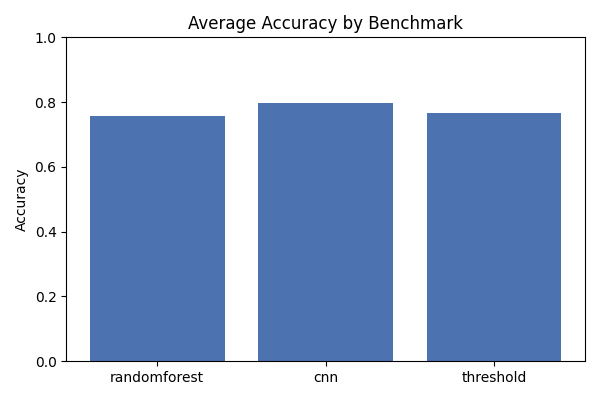
\includegraphics[width=0.8\linewidth]{average_accuracy.png}
\caption{Average CNN accuracy across folds}
\label{fig:avg_accuracy}
\end{figure}

The average accuracy plot aggregates the fold results, making it easy to compare the three pipelines—threshold, random forest, and CNN—and confirms that the CNN leads the pack, followed by the forest.


\noindent \textbf{Summary.} The CNN accuracy per fold and average accuracy charts illustrate how the model generalizes steadily above 80\% across patients, while the performance comparison table ranks the threshold, random forest, and CNN pipelines to show the deep model leading the pack.
The LSTM adds a sequential perspective: by processing windows in temporal order within episodes, it can exploit the pre-ictal → ictal → post-ictal transition that individual-window classifiers ignore.
These plots are based on the latest exported metrics in `out/`.
The threshold classifier baseline achieves an average accuracy of \num{0.766} across folds, while the random forest and CNN improve upon it.


% ==========================================================
\section{Discussion}
Our results show that the CNN consistently outperforms the random forest in accuracy with lower variability across folds.
The deep model effectively captures temporal patterns in EEG signals that simple features cannot represent.
\label{sec:discussion}


% ==========================================================
\section{Conclusion}
We compared a threshold baseline, a feature-based random forest, an end-to-end CNN, and a temporal LSTM for seizure detection in EEG.
The CNN achieved the best performance under patient-level cross-validation, demonstrating the value of expressive, end-to-end models.
The LSTM leverages seizure-level splits to preserve episode integrity and exploit temporal structure; future work will compare it directly against the CNN under matching splits and explore multichannel spatial information combined with longer temporal context.
\label{sec:conclusion}



\newpage

% ==========================================================
\section*{References}
\addcontentsline{toc}{section}{References}
  \begin{enumerate}
   \item Goldberger AL, et al. PhysioBank, PhysioToolkit, and PhysioNet: Components of a New Research Resource for Complex Physiologic Signals. \textit{Circulation}. 2000;101(23):e215--20.
   \item Pedregosa F, et al. Scikit-learn: Machine Learning in Python. \textit{J Mach Learn Res}. 2011;12:2825--30.
   \item Paszke A, et al. PyTorch: An Imperative Style, High-Performance Deep Learning Library. In: \textit{NeurIPS}. 2019.
  \end{enumerate}

% ==========================================================
\appendix

\section{Code extracts}
\label{app:code}

\begin{lstlisting}[language=Python, caption={CNN Model Used}, label=lst:baseline_cnn]
  class SimpleEEGCNN(nn.Module):
      def __init__(self, in_channels: int = 21, n_classes: int = 2) -> None:
          super().__init__()

          self.features = nn.Sequential(
              nn.Conv1d(
                  in_channels=in_channels, out_channels=32, kernel_size=5, padding=2
              ),
              nn.BatchNorm1d(32),
              nn.ReLU(),
              nn.MaxPool1d(kernel_size=2),
              nn.Conv1d(in_channels=32, out_channels=64, kernel_size=5, padding=2),
              nn.BatchNorm1d(64),
              nn.ReLU(),
              nn.MaxPool1d(kernel_size=2),
              nn.Conv1d(in_channels=64, out_channels=128, kernel_size=3, padding=1),
              nn.BatchNorm1d(128),
              nn.ReLU(),
              nn.MaxPool1d(kernel_size=2),
          )

          self.classifier = nn.Sequential(
              nn.Flatten(),
              nn.Linear(128 * 16, 256),
              nn.ReLU(),
              nn.Dropout(0.3),
              nn.Linear(256, n_classes),
          )

      def forward(self, x: torch.Tensor) -> torch.Tensor:
          x = self.features(x)
          x = self.classifier(x)
          return x
\end{lstlisting}
The listing details the architecture described above, including the three convolutional blocks and final classifier layer.

\begin{lstlisting}[language=Python, caption={SeizureLSTM Model}, label=lst:lstm]
class SeizureLSTM(nn.Module):
    def __init__(self, input_size=21, hidden_size=128,
                 num_layers=2, n_classes=2, dropout=0.3):
        super().__init__()
        self.lstm = nn.LSTM(
            input_size=input_size, hidden_size=hidden_size,
            num_layers=num_layers, batch_first=True,
            dropout=dropout if num_layers > 1 else 0.0)
        self.classifier = nn.Linear(hidden_size, n_classes)

    def forward(self, x, lengths=None):
        if lengths is not None:
            x = nn.utils.rnn.pack_padded_sequence(
                x, lengths.cpu(), batch_first=True,
                enforce_sorted=False)
        out, _ = self.lstm(x)
        if lengths is not None:
            out, _ = nn.utils.rnn.pad_packed_sequence(
                out, batch_first=True)
        return self.classifier(out)
\end{lstlisting}
The LSTM processes variable-length episodes of mean-pooled EEG windows and produces per-window seizure/non-seizure logits, using packed sequences to handle padding and seizure-level k-fold to preserve temporal integrity.


\end{document}
